\chapter{El oxígeno del agua}\label{ch:g7:oxygen-in-the-water}

El arroyo de montaña y la charca de verano son los dos ``agua'' --- y
sin embargo la trucha que se lanza por uno se ahogaría en la otra, y la
carpa que prospera en la charca encontraría el arroyo pelado de
comida. La diferencia entre las dos aguas es en buena parte un número
invisible: cuánto \omterm{def:g7:what-is-respiration:respiration}{oxígeno} llevan \omterm{def:g7:oxygen-in-the-water:dissolved}{disuelto}. Este capítulo aprende a
leer, medir y predecir ese número --- y con él, el mapa de la vida
acuática.

\section{El oxígeno disuelto, una reserva escasa}

\begin{definition}[Oxígeno disuelto]\label{def:g7:oxygen-in-the-water:dissolved}
El agua lleva \omterm{def:g7:what-is-respiration:respiration}{oxígeno} igual que el té con azúcar lleva azúcar --- sin
verse, \emph{disuelto}\index{oxígeno disuelto}. La cantidad es
diminuta: un litro de agua bien aireada lleva unos \qty{10}{mg} de
\omterm{def:g7:what-is-respiration:respiration}{oxígeno}, unas treinta veces menos que un litro de aire. Todas las
\omterm{def:g7:how-animals-breathe:four}{branquias} y todos los que respiran bajo el agua del
\cref{ch:g7:how-animals-breathe} tiran de esta única reserva escasa
(\cref{prop:g7:what-is-respiration:habitats}).
\end{definition}

\begin{proposition}[Qué llena la reserva]\label{prop:g7:oxygen-in-the-water:fills}
Dos proveedores reponen el \omterm{def:g7:what-is-respiration:respiration}{oxígeno} de un agua:
\begin{enumerate}
  \item el \emph{aire de arriba}: el \omterm{def:g7:what-is-respiration:respiration}{oxígeno} se disuelve en la
        superficie --- más deprisa donde el agua se remueve, salpica y
        hace espuma (rápidos, cascadas, olas, lluvia);
  \item las \emph{\omterm{def:g5:food-webs:roles}{productoras} de abajo}: de día, las \omterm{def:g1:plants-around-us:plant}{plantas} acuáticas
        y las \omterm{def:g5:first-look-at-cells:cell}{células} verdes sueltas sueltan \omterm{def:g7:what-is-respiration:respiration}{oxígeno} al agua mientras
        fabrican (\cref{rem:g6:plants-are-producers:gas}).
\end{enumerate}
\end{proposition}
\admitted

\begin{proposition}[Qué la vacía y cuánto puede llevar]\label{prop:g7:oxygen-in-the-water:drains}
La reserva la vacían \emph{todos los que respiran} --- los \omterm{def:g1:animals-around-us:animal}{animales},
las \omterm{def:g1:plants-around-us:plant}{plantas} de noche y, sobre todo, los \omterm{def:g6:decomposers-and-soil:decomposers}{descomponedores} cuando hay
mucha materia muerta que comer (el octavo tarro del
\cref{pb:g7:what-is-respiration:1}). Y el techo se mueve: el agua
\emph{fría} puede llevar bastante más \omterm{def:g7:oxygen-in-the-water:dissolved}{oxígeno disuelto} que la caliente
--- un arroyo a \qty{5}{\degreeCelsius} lleva la mitad más que una
charca a \qty{25}{\degreeCelsius}. El calor aprieta por dos lados:
menos \omterm{def:g7:what-is-respiration:respiration}{oxígeno} llevado, mientras todos los ruidos de motor
(\cref{ex:g7:what-is-respiration:demand}) corren más deprisa.
\end{proposition}
\admitted

\begin{example}[El arroyo frente a la charca]\label{ex:g7:oxygen-in-the-water:streampond}
Las dos aguas se leen ahora como dos contabilidades. El arroyo de
montaña: frío (techo alto), batido y blanco sobre cada peñasco (relleno
rápido) --- \omterm{def:g7:what-is-respiration:respiration}{oxígeno} cerca del techo todo el año. La charca de verano:
caliente (techo bajo), quieta (relleno lento), rica en barro y en
materia muerta (\omterm{def:g6:decomposers-and-soil:decomposers}{descomponedores} hambrientos) --- \omterm{def:g7:what-is-respiration:respiration}{oxígeno} rozando el
fondo, y peor en las horas pequeñas antes del amanecer, cuando las
\omterm{def:g1:plants-around-us:plant}{plantas} llevan toda la noche respirando sin ninguna fabricación diurna
que las compense.
\end{example}

\begin{omfigure}
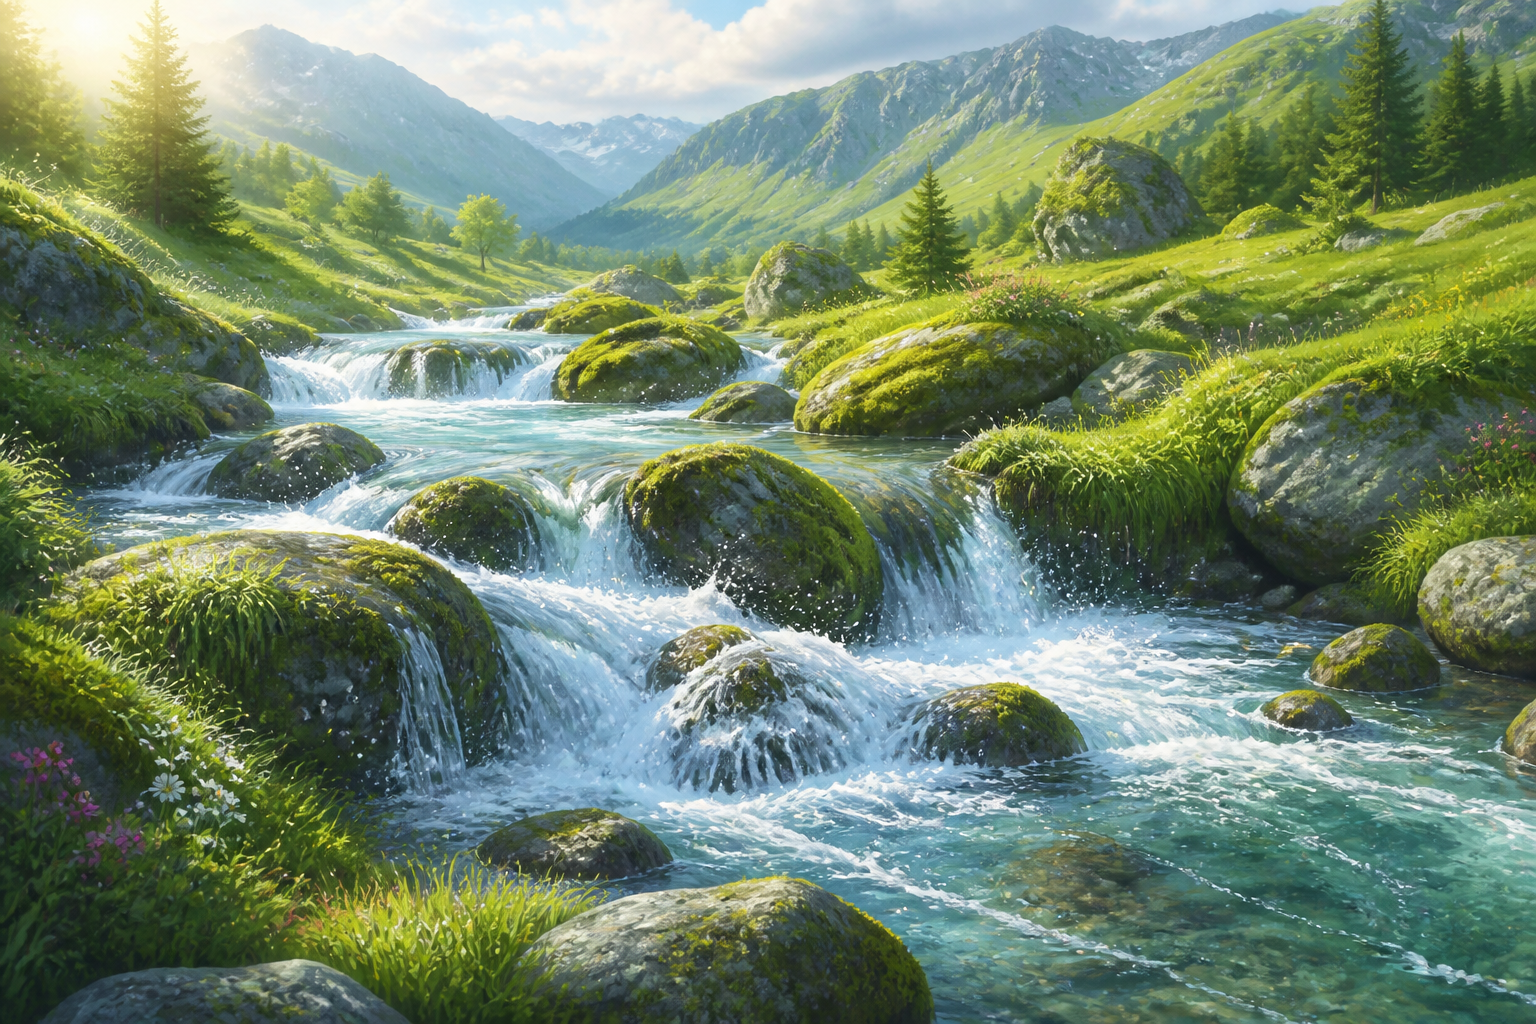
\includegraphics[width=0.62\linewidth]{images/book1/ai/g7-oxygen-stream.png}

{\small El extremo rico en \omterm{def:g7:what-is-respiration:respiration}{oxígeno}: agua fría, batida y blanca en cada
peñasco --- un techo alto que se rellena sin parar.}
\end{omfigure}

\begin{omfigure}
\begin{tikzpicture}
\begin{axis}[omaxis,
    width=9.6cm, height=5.6cm,
    xlabel={hora del día}, ylabel={oxígeno disuelto (mg/L)},
    xmin=0, xmax=27, ymin=0, ymax=14,
    xtick={0,6,12,18,24},
    ytick={4,8,12},
    ]
  % stream: flat high
  \addplot[very thick, omDef] coordinates {
    (0,10.6) (6,10.7) (12,10.4) (18,10.5) (24,10.6)
  };
  % pond: sinusoidal-ish, low before dawn, peak late afternoon
  \addplot[very thick, omThm, smooth] coordinates {
    (0,4.4) (3,3.4) (6,3.0) (9,5.2) (12,7.8) (15,9.4)
    (17,9.8) (20,7.4) (24,4.6)
  };
  \node[font=\footnotesize, omDef] at (axis cs:4.6,12.1)
    {arroyo de montaña};
  \node[font=\footnotesize, omThm] at (axis cs:8.2,1.6)
    {charca de verano};
\end{axis}
\end{tikzpicture}

{\small Un día de \omterm{def:g7:oxygen-in-the-water:dissolved}{oxígeno disuelto}. El arroyo frío y batido se mantiene
firme cerca de su techo alto; la charca caliente cabalga a sus
\omterm{def:g5:food-webs:roles}{productoras} --- sube a lo largo del día y se hunde durante la noche
hasta un mínimo al amanecer.}
\end{omfigure}

\begin{example}[Leer la curva de la charca]\label{ex:g7:oxygen-in-the-water:curve}
La onda diaria de la charca es la
\cref{rem:g6:plants-are-producers:gas} dibujada como datos: el amanecer
pone en marcha la fabricación de las \omterm{def:g5:food-webs:roles}{productoras} y la curva sube; a
última hora de la tarde llega al máximo; la noche deja a todos los que
respiran tirando de la reserva sin más proveedor que la superficie
quieta --- y la curva se desliza hasta su mínimo del amanecer. Las
mortandades de \omterm{prop:g3:sorting-living-things:groups}{peces} en charcas invadidas de vegetación ocurren al
amanecer, y ahora ya sabes por qué.
\end{example}

\section{El mapa de los habitantes}

\begin{proposition}[El oxígeno dibuja el mapa]\label{prop:g7:oxygen-in-the-water:map}
Como las \omterm{def:g5:biodiversity:species}{especies} se diferencian en sus necesidades de \omterm{def:g7:what-is-respiration:respiration}{oxígeno}, el
número del \omterm{def:g7:oxygen-in-the-water:dissolved}{disuelto} cartografía a los habitantes (la
\cref{prop:g6:exploring-our-environment:decide}, bajo el agua):
\begin{itemize}
  \item las \omterm{def:g5:biodiversity:species}{especies} \emph{exigentes} --- la trucha, las larvas de
        efímera con sus penachos branquiales agitándose
        (\cref{pb:g7:how-animals-breathe:1}) --- solo viven en aguas
        frías, batidas y ricas en \omterm{def:g7:what-is-respiration:respiration}{oxígeno};
  \item las \omterm{def:g5:biodiversity:species}{especies} \emph{tolerantes} --- la carpa, muchos caracoles
        de charca, las larvas con cola de rata y su tubo hasta la
        superficie --- se apañan en aguas cálidas, quietas y más pobres;
  \item así que el censo se lee al revés: si encuentras larvas de
        efímera bajo las piedras, el agua es buena; si solo encuentras
        larvas con tubo y tragadores de aire, es mala.
\end{itemize}
Los guardas de río censan la vida pequeña justamente por eso: los
habitantes son un registro de los peores días recientes del agua, y una
sola lectura de sonda se los puede perder.
\end{proposition}
\admitted

\begin{example}[La historia de los residuos orgánicos]\label{ex:g7:oxygen-in-the-water:waste}
Los residuos sin tratar de un pueblo --- ricos en \omterm{def:g6:plants-are-producers:matter}{materia orgánica} ---
llegan a un arroyo limpio. Aguas abajo de la tubería, los
\omterm{def:g6:decomposers-and-soil:decomposers}{descomponedores} se dan un banquete y se multiplican
(\cref{def:g6:decomposers-and-soil:decomposers}), y su \omterm{def:g7:what-is-respiration:respiration}{respiración}
masiva vacía el \omterm{def:g7:what-is-respiration:respiration}{oxígeno}: las truchas y las larvas de efímera
desaparecen, se hacen con el sitio las tolerantes de tubo y, más abajo
todavía --- consumidos los residuos y reaireada el agua sobre los
rápidos ---, vuelven las \omterm{def:g5:biodiversity:species}{especies} exigentes. La contaminación era
\omterm{def:g6:plants-are-producers:matter}{materia orgánica}; el asesino fue el hambre de \omterm{def:g7:what-is-respiration:respiration}{oxígeno}; y el mapa lo
registró todo.
\end{example}

\begin{method}[Juzgar un agua]\label{met:g7:oxygen-in-the-water:judge}
Para juzgar un arroyo o una charca:
\begin{enumerate}
  \item mide o estima los proveedores: \omterm{def:g6:exploring-our-environment:conditions}{temperatura}, agitación,
        crecimiento verde;
  \item pesa los desagües: barro y materia muerta, hacinamiento,
        cualquier entrada de residuos orgánicos;
  \item censa la vida pequeña bajo las piedras y entre las hierbas ---
        ¿hay \omterm{def:g5:biodiversity:species}{especies} exigentes o solo tolerantes?
  \item si tomas la muestra a una sola hora, acuérdate de la curva de
        la charca: una buena lectura de tarde puede esconder un
        amanecer mortal.
\end{enumerate}
\end{method}

\section{Ejercicios}

\begin{exercise}[$\star$]\label{exo:g7:oxygen-in-the-water:1}
¿Cuánto \omterm{def:g7:what-is-respiration:respiration}{oxígeno} lleva más o menos un litro de agua bien aireada y cómo
se compara eso con el aire?
\end{exercise}

\begin{exercise}[$\star$]\label{exo:g7:oxygen-in-the-water:2}
Nombra los dos proveedores del \omterm{def:g7:what-is-respiration:respiration}{oxígeno} de un agua y la condición en la
que cada uno suministra más deprisa.
\end{exercise}

\begin{exercise}[$\star$]\label{exo:g7:oxygen-in-the-water:3}
Nombra tres desagües de la reserva. ¿Cuál se hace enorme cuando abunda
la materia muerta?
\end{exercise}

\begin{exercise}[$\star$]\label{exo:g7:oxygen-in-the-water:4}
Enuncia el doble apretón del calor sobre los que respiran en el agua.
\end{exercise}

\begin{exercise}[$\star$]\label{exo:g7:oxygen-in-the-water:5}
¿Por qué llega la curva de \omterm{def:g7:what-is-respiration:respiration}{oxígeno} de la charca a su máximo a última
hora de la tarde y a su mínimo al amanecer?
\end{exercise}

\begin{exercise}[$\star$]\label{exo:g7:oxygen-in-the-water:6}
¿Qué dos hallazgos de un censo marcan un agua rica en \omterm{def:g7:what-is-respiration:respiration}{oxígeno} y cuáles
marcan una pobre?
\end{exercise}

\begin{exercise}[$\star\star$]\label{exo:g7:oxygen-in-the-water:7}
Explícale la mortandad de \omterm{prop:g3:sorting-living-things:groups}{peces} al amanecer del
\cref{ex:g7:oxygen-in-the-water:curve} a la dueña de una charca --- y
propón un remedio a partir de cada proveedor de la
\cref{prop:g7:oxygen-in-the-water:fills}.
\end{exercise}

\begin{exercise}[$\star\star$]\label{exo:g7:oxygen-in-the-water:8}
Vuelve a contar el \cref{ex:g7:oxygen-in-the-water:waste} como una
cadena: entran los residuos, ¿y luego?, ¿y luego? --- y ¿por qué se cura
el arroyo aguas abajo?
\end{exercise}

\begin{exercise}[$\star\star$]\label{exo:g7:oxygen-in-the-water:9}
¿Por qué se fían los guardas de río más del censo de vida pequeña que
de una sola lectura de sonda? Usa la idea de ``los peores días
recientes''.
\end{exercise}

\begin{exercise}[$\star\star$]\label{exo:g7:oxygen-in-the-water:10}
Una charca de jardín se pone verde de sopa de guisantes y después
aguanta una semana calurosa y sin viento. Sigue el peligro con las dos
proposiciones --- y di cuándo debería su dueño poner la fuente a tope.
\end{exercise}

\begin{exercise}[$\star\star$]\label{exo:g7:oxygen-in-the-water:11}
Las piscifactorías de trucha se construyen en ríos fríos con azudes y
canales de agua salpicando, nunca en lagos cálidos y quietos. Justifica
todas las partes de la frase.
\end{exercise}

\begin{exercise}[$\star\star\star$]\label{exo:g7:oxygen-in-the-water:12}
``En el agua, el \omterm{def:g7:what-is-respiration:respiration}{oxígeno} es la moneda; la \omterm{def:g6:exploring-our-environment:conditions}{temperatura} fija la cantidad
de dinero; los \omterm{def:g6:decomposers-and-soil:decomposers}{descomponedores} son los que más gastan''. Traduce cada
parte a las afirmaciones llanas de este capítulo, citando una
proposición o un ejemplo para cada una.
\end{exercise}

\section{Problema: El anuario del guarda}

\begin{problem}[{Problema de fin de semana --- un río, cuatro
estaciones y un año de lecturas}]\label{pb:g7:oxygen-in-the-water:1}
Un guarda de río lleva un anuario de cuatro estaciones: K1, un rápido
frío justo debajo de un azud; K2, un tramo lento y cálido entre pastos;
K3, justo debajo de la tubería de residuos de una quesería; y K4, dos
kilómetros más abajo, pasado un largo rápido pedregoso. Cada estación
recibe lecturas de sonda y un censo de vida pequeña.

\medskip\noindent\textbf{Parte I --- Leer las estaciones.}
\begin{enumerate}
  \item K1 marca \qty{11}{mg/L} a \qty{8}{\degreeCelsius}; K2 marca
        \qty{7}{mg/L} a \qty{22}{\degreeCelsius}. Atribuye la
        diferencia a los proveedores y a los techos que corresponden.
  \item Censo de K1: alevines de trucha y larvas de efímera. El de K2:
        carpas, caracoles de charca y larvas con cola de rata.
        Interpreta los dos con la
        \cref{prop:g7:oxygen-in-the-water:map}.
  \item K3 marca \qty{3}{mg/L} aunque el agua no está más caliente que
        en K2. Nombra el desagüe y a los trabajadores que hay detrás.
  \item K4 marca \qty{9}{mg/L} y su censo vuelve a enseñar larvas de
        efímera. Explica la recuperación con los dos proveedores y con
        el destino de los residuos.
\end{enumerate}

\medskip\noindent\textbf{Parte II --- Los ritmos del año.}
\begin{enumerate}[resume]
  \item Las lecturas de K2 al amanecer en agosto bajan a \qty{4}{mg/L}
        mientras que las de la tarde llegan a \qty{9}{mg/L}. Dibuja o
        describe su curva diaria y nombra los dos procesos que se van
        turnando.
  \item Las lecturas de enero en K2 son más estables y más altas que
        las de agosto, aunque el tramo de los pastos sigue igual de
        quieto. Da las dos razones invernales.
  \item Se anuncian quince días calurosos y sin viento. Ordena las
        cuatro estaciones por riesgo de mortandad de \omterm{prop:g3:sorting-living-things:groups}{peces}, con una
        razón para cada una.
  \item La guarda programa sus visitas de sonda de agosto para justo
        antes de que salga el sol. Defiende el horario.
\end{enumerate}

\medskip\noindent\textbf{Parte III --- Veredictos y remedios.}
\begin{enumerate}[resume]
  \item La quesería instala un tratamiento que quita casi toda la
        \omterm{def:g6:plants-are-producers:matter}{materia orgánica} de su vertido. Predice la sonda y el censo de
        K3 un año después, en orden de recuperación.
  \item Un propietario propone talar los árboles de la orilla de K2
        ``para que entre más \omterm{def:g6:exploring-our-environment:conditions}{luz} y se haga más \omterm{def:g7:what-is-respiration:respiration}{oxígeno}''. Sopesa la
        propuesta: ¿qué hace además la sombra, según la
        \cref{prop:g7:oxygen-in-the-water:drains}, y qué responderías?
  \item El censo encuentra larvas de efímera en una estación cuya única
        lectura de sonda de la tarde parece mediocre. ¿A qué testigo le
        crees sobre la temporada entera y por qué?
  \item Cierra el anuario con la regla en una frase de la guarda para
        todo el río, usando \emph{frío}, \emph{removido} y \emph{sin
        carga} (de residuos orgánicos).
\end{enumerate}
\end{problem}
